\documentclass[letterpaper,10pt]{article}
\usepackage[top=2cm, bottom=1.5cm, left=1cm, right=1cm]{geometry}
\usepackage{amsmath, amssymb, amsthm, graphicx, enumitem}
\usepackage{fancyhdr}
\pagestyle{fancy}

\lhead{\today}
\chead{MATH 740 Assignment 1}
\rhead{Justin Hood}

\newcommand{\Z}{\mathbb{Z}}
\newcommand{\Q}{\mathbb{Q}}
\newcommand{\R}{\mathbb{R}}
\newcommand{\C}{\mathbb{C}}
\newtheorem{lem}{Lemma}

\begin{document}
\begin{description}
\item[Problem 1.2] \hfill \\
We consider the data contained in the following table:
\begin{center}
\begin{tabular}{c|rrrrrrrrrr}
$x_1$ & 1 & 2 & 3 & 3 & 4 & 5 & 6 & 8 & 9 & 11\\\hline
$x_2$ & 18.95 & 19.00 & 17.95 & 15.54 & 14.00 & 12.95 & 8.94 & 7.49 & 6.00 & 3.99
\end{tabular}
\end{center}
\begin{enumerate}[label=(\alph*)]
\item To begin, we construct a scatter plot with marginal histograms to get a sense of the data. This is shown below,
\begin{center}
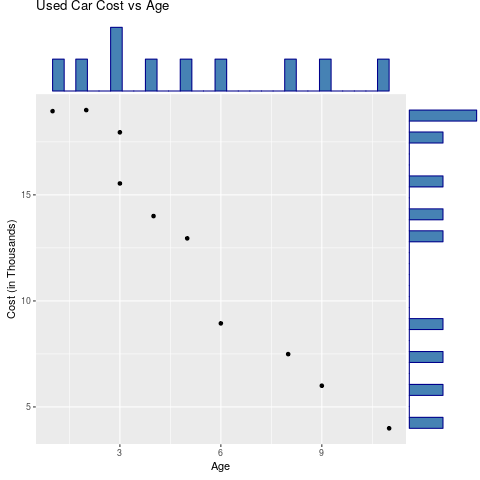
\includegraphics[scale=0.75]{12scatter.png}
\end{center}
\item Based on the trend in the data, i.e. the negative slope of the data, we may concude that the sign of the covariance of the data is negative.
\item Using $R$, we compute the means $\bar{x}_1,\ \bar{x}_2$ to be,
\[\bar{x}_1=5.2,\ \bar{x}_2=12.481\]
Next, we compute the sample variances $s_{11}$ and $s_{22}$ using the formula,
\[s_{kk}=\frac{1}{n}\sum_{j=1}^n(x_{jk}-\bar{x}_k)^2\]
Thus,
\[s_{11}=\frac{1}{10}\sum_{j=1}^{10}(x_{j1}-\bar{x}_1)^2=9.56\]
\[s_{22}=\frac{1}{10}\sum_{j=1}^{10}(x_{j2}-\bar{x}_2)^2=27.768929\]
Next, we compute the sample covariance $s_{12}$ using the formula,
\[s_{ik}=\frac{1}{n}\sum_{j=1}^n(x_{ji}-\bar{x}_i)(x_{jk}-\bar{x}_k)\]
Thus,
\[s_{12}=\frac{1}{10}\sum_{j=1}^{10}(x_{ji}-5.2)(x_{jk}-12.481)=-15.9392=s_{21}\]
Finally, we compute the sample correlation coefficient $r_{12}$ using the formula,
\[s_{ik}=\frac{s_{ik}}{\sqrt{s_{ii}}\sqrt{s_{kk}}}=\frac{-15.9392}{\sqrt{9.56}\sqrt{27.768929}}=-0.9782684\]
\item The above data may be succinctly summarized by the following arrays,
\begin{align*}
\bar{\textbf{x}} &= \begin{bmatrix}
5.2\\12.481
\end{bmatrix}\\
\textbf{S}_{10} &= \begin{bmatrix}
9.56 & -15.9392\\ -15.9392 & 27.76893
\end{bmatrix}\\
\textbf{R} &= \begin{bmatrix}
1 & -0.9782684\\-0.9782684 & 1
\end{bmatrix}
\end{align*}
\end{enumerate}
\item[Problem 1.4]\hfill \\
Using the data from the provided table, we compute the scatter and marginal dot diagrams  for the variables $x_1$ and $x_2$ as follows:
\begin{enumerate}[label=(\alph*)]
\item Plotting the data in the form of a scatter plot concerning the variables $x_1$ and $x_2$, we obtain the following,
\begin{center}
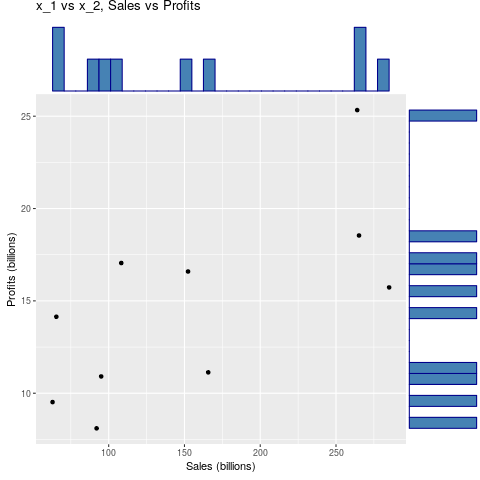
\includegraphics[scale=0.75]{14scatter.png}
\end{center}
Based on this plot, we see that the covariance between the variables seems to be positive, but the correlation between them seems fairly weak.
\item We shall now compute the relevant summary statistics below using $R$,
\begin{center}
\begin{tabular}{c|r}
Statistic & Value\\\hline
$\bar{x}_1$ & 155.603\\
$\bar{x}_2$ & 14.704\\
$s_{11}$ & 6728.808\\
$s_{22}$ & 23.571284\\
$s_{12}$ & 273.256758\\
$r_{12}$ & 0.686136\\
\end{tabular}
\end{center}
As noted in part (a), we see that the correlation value is not very close to $1$. This makes sense, as the data shows a decent amount of variance around a hypothetical mean line.
\end{enumerate}
\item[Problem 1.5]\hfill\\
Continuing with the analysis from problem 1.4, we now consider the scatter plot and marginal diagrams for $(x_2,x_3)$ and $(x_1,x_3)$. These plots follow,
\begin{center}
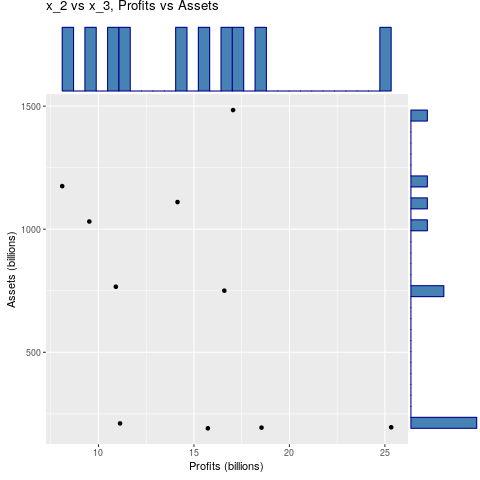
\includegraphics[scale=0.75]{1523scatter.png}
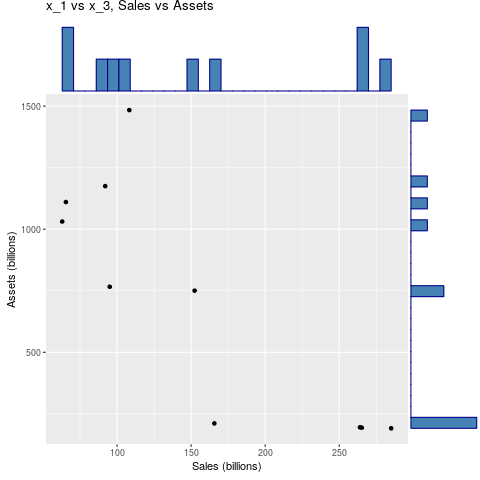
\includegraphics[scale=0.75]{1513scatter.png}
\end{center}
For both of these plots, the overall trend is difficult to discern. For the plot of $(x_2,x_3)$, it is nearly impossible to tell if the data has a positive or negative covariance. For the plot of $(x_1,x_3)$, the covariance appears to be negative, but again, it is difficult to tell.
\item We shall now compute the relevant summary statistics in array form using $R$. The results are,
\begin{align*}
\bar{\textbf{x}} &= \begin{bmatrix}
155.603\\14.704\\710.911
\end{bmatrix}\\
\textbf{S}_{10} &= \begin{bmatrix}
6728.808 & 273.2568 & -32018.36\\
273.2568 & 23.57128 & -948.4447\\
-32018.36 & -948.4447 & 213348.8
\end{bmatrix} \\
\textbf{R} &= \begin{bmatrix}
1 & 0.686136 & -0.8450549\\
0.686136 & 1 & -0.4229366\\
-0.8450549 & -0.4229366 & 1
\end{bmatrix}
\end{align*}
\item[Problem 1.17]\hfill \\
The summary statistics computed in $R$ follow,
\begin{align*}
\bar{\textbf{x}} &= \begin{bmatrix}
11.35778\\23.11852\\51.98907\\2.022407\\4.189444\\9.080741\\153.6193
\end{bmatrix}\\
\textbf{S}_{54} &= \begin{bmatrix}
0.1524395 & 0.3381800  &  0.8747905  &  1.631432  &   4.940259  &  13.77310 &   255.2349\\
0.3381800 &  0.8471052  &  2.1522283  &  3.896436  &  11.940506  &  32.64507  &  611.5604\\
0.8747905 &  2.1522283  &  6.6205417 &  10.706467  &  29.984858  &  84.02360  & 1702.1086\\
1.6314321 &  3.8964362  & 10.7064671 &  26.665802  &  75.664815 &  216.87358  & 4309.4464\\
4.9402593 & 11.9405062   & 29.9848580 &  75.664815 &  262.112222 &  763.74815 & 12507.4252\\
13.7730988 & 32.6450658 &  84.0235967 & 216.873580  & 763.748148 & 2348.81136 & 37828.1886\\
255.2349012 & 611.5603786 & 1702.1086255 & 4309.446420 & 12507.425185 & 37828.18864 & 954954.5314
\end{bmatrix}\\
\textbf{R} &= \begin{bmatrix}
1.0000000 & 0.9410886 & 0.8707802 & 0.8091758 & 0.7815510 & 0.7278784 & 0.6689597\\
0.9410886 & 1.0000000 & 0.9088096 & 0.8198258 & 0.8013282 & 0.7318546 & 0.6799537\\
0.8707802 & 0.9088096 & 1.0000000 & 0.8057904 & 0.7197996 & 0.6737991 & 0.6769384\\
0.8091758 & 0.8198258 & 0.8057904 & 1.0000000 & 0.9050509 & 0.8665732 & 0.8539900\\
0.7815510 & 0.8013282 & 0.7197996 & 0.9050509 & 1.0000000 & 0.9733801 & 0.7905565\\
0.7278784 & 0.7318546 & 0.6737991 & 0.8665732 & 0.9733801 & 1.0000000 & 0.7987302\\
0.6689597 & 0.6799537 & 0.6769384 & 0.8539900 & 0.7905565 & 0.7987302 & 1.0000000
\end{bmatrix}
\end{align*}
From this matrix of correlation coefficients, we see that as we increase in the distance of the race, the correlation declines between the shorter and longer races. Because this correlation declines, we see that the linearity between the categories decreases, which makes sense, as the times for the marathon will exhibit a much larger variation in time than the 100 meter. This is because the amount of time required to run a marathon is many orders of magnitude larger than the time that top runners require to run a 100m sprint. We note that it is not necessary to convert the times for the longer records to seconds, as these computations are independent of scalar multiplication, and the same results will be obtained.
\item[Problem 1.18]\hfill\\
We shall perform the same analysis as before, but on the data converted to the speeds in $m/s$ of the records as opposed to the times. After converting all of the records to seconds, and then into speed using the relation $d/t=r$, we compute the relevant statistics again as follows,
\begin{align*}
\bar{\textbf{x}} &= \begin{bmatrix}
8.815\\8.664\\7.712\\6.604\\5.990\\5.543\\4.620  
\end{bmatrix}\\
\textbf{S}_{54} &= \begin{bmatrix}
0.08886163 & 0.09383586 & 0.09488221 & 0.06385913 & 0.08069721 & 0.09043587 & 0.07959802\\
0.09383586 & 0.11254789 & 0.11176120 & 0.07353737 & 0.09424082 & 0.10348392 & 0.09158236\\
0.09488221 & 0.11176120 & 0.13523721 & 0.07944200 & 0.09367553 & 0.10631059 & 0.09999405\\
0.06385913 & 0.07353737 & 0.07944200 & 0.07216131 & 0.08485322 & 0.09790735 & 0.09255923\\
0.08069721 & 0.09424082 & 0.09367553 & 0.08485322 & 0.12154716 & 0.14105343 & 0.11626411\\
0.09043587 & 0.10348392 & 0.10631059 & 0.09790735 & 0.14105343 & 0.17331425 & 0.14384635\\
0.07959802 & 0.09158236 & 0.09999405 & 0.09255923 & 0.11626411 & 0.14384635 & 0.16362679
\end{bmatrix}\\
\textbf{R} &= \begin{bmatrix}
1.0000000 & 0.9383028 & 0.8655248 & 0.7974687 & 0.7764777 & 0.7287297 & 0.6601124\\
0.9383028 & 1.0000000 & 0.9058875 & 0.8159945 & 0.8057456 & 0.7409469 & 0.6748635\\
0.8655248 & 0.9058875 & 1.0000000 & 0.8041737 & 0.7306437 & 0.6944025 & 0.6722005\\
0.7974687 & 0.8159945 & 0.8041737 & 1.0000000 & 0.9060324 & 0.8754795 & 0.8518052\\
0.7764777 & 0.8057456 & 0.7306437 & 0.9060324 & 1.0000000 & 0.9718385 & 0.8244153\\
0.7287297 & 0.7409469 & 0.6944025 & 0.8754795 & 0.9718385 & 1.0000000 & 0.8541900\\
0.6601124 & 0.6748635 & 0.6722005 & 0.8518052 & 0.8244153 & 0.8541900 & 1.0000000
\end{bmatrix}
\end{align*}
Again, we see that the correlation coefficients decrease in magnitude as the distance increases along the rows of the matrix. This too makes sense, because the speed that may be maintained for a 100m dash is much higher than the speed that may be maintained for a marathon. So, for the same country data, we note that the speed for the 100m is much higher than the marathon speed. As noted in problem 1.17, we came to the conclusion that the amount of time requred to run a marathon was many orders of magnitude higher than that of the 100m dash. Using this notion, if we consider the speeds of the races, we see that the mean speeds are of similar magnitude. This is due to the relation of distance and time for speed. Since the increase in distance corresponds to an increase in time, we see that the speeds are all of relative similarity.
\end{description}
\end{document}
